17. 下边这幅漫画对于我们认识人与自然关系的警示意义在于
\begin{center}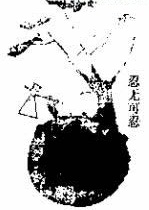
\includegraphics[height=4cm]{17.jpg}\end{center}
\begin{choices}
	\choice0 人类过分陶醉于对自然界的胜利将受到自然界的报复
	\choice0 人与自然关系的紧张来自于不当的人类实践方式
	\choice0 人与自然的关系本质上是对立的
	\choice0 人类依附于自然是摆脱自身困境的根本出路
\end{choices}
18. 19世纪英国作家惠兹里特说:“一个除了书本以外一无所知的纯粹学者,必然对书本也是无知的。”与这句话在内涵上相一致的名言还有
\begin{choices}
	\choice0 纸上得来终觉浅,绝知此事要躬行
	\choice0 尽信书,则不如无书
	\choice0 感觉到了的东西我们不能离可理解它,只有理解了的东西才能更深刻地感觉它
	\choice0 饱经风霜的老人与缺乏阅历的少年对同一句格言的理解是不同的
\end{choices}
19. 马克思主义哲学中的辩证法、认识论、历史观在本质上是一致的,体现这种一致性的公式有
\begin{choices}
	\choice0 个别——一般——个别
	\choice0 实践——认识——实践
	\choice0 群众——领导——群众
	\choice0 团结——批评——团结
\end{choices}
20. 随着科学技术和经济全球化的发展,人类的交往活动日益普遍和深化,交往作为人类特有的活动和存在方式,对社会发展具有越来越重要的作用。主要表现在
\begin{choices}
	\choice0 交往促进生产力的发展
	\choice0 交往推动社会关系的变革和改善
	\choice0 交往是科学文化传承和发展的重要途径
	\choice0 交往促进人自身的发展
\end{choices}
21. 同一劳动在同一时间内,当部门劳动生产率提高时会使
\begin{choices}
	\choice0 单位商品的价值量降低
	\choice0 商品的使用价值量增加
	\choice0 单位商品的价值量不变
	\choice0 单位商品的价值量提高
\end{choices}
22. 通过对社会资本简单再生产实现过程中交换关系的分析,可以看出
\begin{choices}
	\choice0 Ⅰc是通过第Ⅰ部类内部交换实现的
	\choice0 Ⅱ(v+m)是通过第Ⅱ部类内部交换实现的
	\choice0 Ⅰ(v+m)是通过和Ⅱ(v+m)交换实现的
	\choice0 Ⅰ(v+m)是通过和Ⅱc交换实现的
\end{choices}
23. 为了保持物价总水平的稳定,国家实施宏观调控可以采取的货币政策手段有
\begin{choices}
	\choice0 调整存贷款基准利率
	\choice0 调整法定存款准备金库
	\choice0 实施物价补贴
	\choice0 调整再贴现率
\end{choices}
24. 为完善社会主义个人收入分配制度,确立生产要素按贡献参与分配是基于
\begin{choices}
	\choice0 各种生产要素都能创造价值
	\choice0 要素所有权关系在经济上的体现
	\choice0 市场经济配置资源的内在要求
	\choice0 各种生产要素都具有价值
\end{choices}
25. 在中国共产党的历史上,对毛泽东思想作出系统概括和阐述的党的文献有
\begin{choices}
	\choice0 《关于若干历史问题的决议》
	\choice0 刘少奇在七大上所作的《关于修改党的章程的报告》
	\choice0 邓小平在八大上所作的《关于修改党的章程的报告》
	\choice0 《关于建国以来党的若干历史问题的决议》
\end{choices}
26. 关于民主革命时期富农身份的界定,下列选项中正确的有
\begin{choices}
	\choice0 剥削雇农的剩余劳动,是农村中的资产阶级
	\choice0 既是劳动者,又是剥削者
	\choice0 自身不劳动,出租土地并放高利贷
	\choice0 对雇农的剥削带有浓厚的半封建性
\end{choices}
27. 新中国建立之际,毛泽东提出的外交方针有
\begin{choices}
	\choice0 “一边倒”
	\choice0 “反霸权主义”
	\choice0 “打扫干净屋子再请客”
	\choice0 “另起炉灶”
\end{choices}
28. 党的十七大报告指出,深入贯彻落实科学发展观,必须坚持
\begin{choices}
	\choice0 把发展作为党执政兴国的第一要务
	\choice0 以人为本
	\choice0 全面协调可持续发展
	\choice0 统筹兼顾
\end{choices}
29. 党的十七大报告指出,十一届三中全会以来,中国共产党坚持马克思主义的思想路线,不断探索和回答的重大理论和实际问题是
\begin{choices}
	\choice0 什么是社会主义、怎样建设社会主义
	\choice0 什么是现代化、怎样建设现代化
	\choice0 建设什么样的党、怎样建设党
	\choice0 实现什么样的发展、怎样发展
\end{choices}
30. 人民代表大会制度是我国的根本政治制度,这是因为
\begin{choices}
	\choice0 它直接体现我国人民民主专政的国家性质
	\choice0 它能从根本上保证人民当家作主的权力
	\choice0 它在制定国家其他各种制度中起着决定性的作用
	\choice0 它能使广大人民在国家政治生活中直接行使民主权力
\end{choices}
31. 2005年,胡锦涛主席就新形势下发展两岸关系提出的原则性意见是
\begin{choices}
	\choice0 坚持一个中国的原则决不动摇
	\choice0 争取和平统一的努力决不放弃
	\choice0 贯彻寄希望于台湾人民的方针决不改变
	\choice0 反对“台独”分裂活动决不妥协
\end{choices}
32. 党的十七大报告指出,高举中国特色社会主义伟大旗帜,最根本的就是要坚持
\begin{choices}
	\choice0 中国特色社会主义道路
	\choice0 实事求是的思想路线
	\choice0 中国特色社会主义理论体系
	\choice0 改革开放的战略方针
\end{choices}
33. 2007年2月,胡锦涛主席在与苏丹总统巴希尔的会谈中提出,处理达尔富尔问题应该
\begin{choices}
	\choice0 尊重苏丹的主权和领土完整
	\choice0 发挥非盟、联合国的建设性作用
	\choice0 有利于促进达尔富尔地区局势稳定
	\choice0 通过和平方式解决问题
\end{choices}
\vspace{6pt}
